\section{実験方法}
本実験では以下の3つの実験を行った.

\renewcommand{\theenumi}{\Roman{enumi}}
\begin{enumerate}
    \item 平面き裂:6デシベルドロップ法
    \item 欠陥評価:AVG線図
    \item 最先端超音波探傷の理解
\end{enumerate}

実験I,IIで用いた実験装置を図\ref{fig:実験装置}に示す.パルサーは探触子を振動させ超音波を発信する装置であり,レシーバーは反射した超音波を探触子で電気信号に表示する装置である.探触子は周波数$f = 5\mathrm{MHz}$,直径$D = 6.3\mathrm{mm}$のものを使用した.
\begin{figure}[htbp]
    \centering %中央揃え
    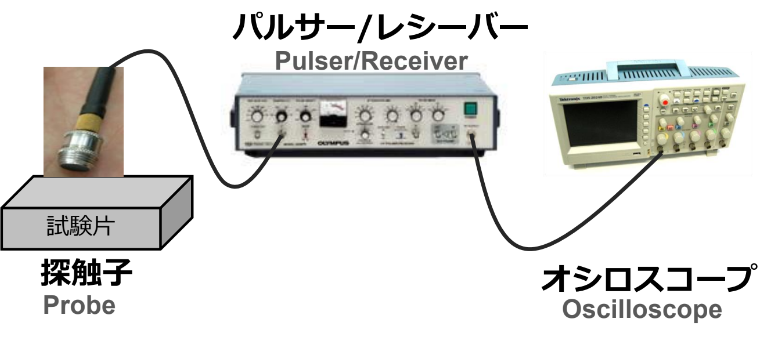
\includegraphics[width=100truemm,clip]{fig/実験装置.png}
    \caption{Experimental apparatus in Experiments I and II.}
    \label{fig:実験装置}
\end{figure}

\renewcommand{\theenumi}{\arabic{enumi}}
\subsection{実験I}
図\ref{fig:実験I}に計測した試験体の形状を示す.実験手順を以下に示す.
\begin{enumerate}
    \item 試験体表面にグリスを塗布した.
    \item 探触子を試験体表面に当てて,オシロスコープのエコーを確認した.
    \item 第1回エコーが送信パルスに対して,大きく変わらない場所で探触子を静止し,オシロスコープの波形を記録した.
    \item オシロスコープの波形から図\ref{fig:試験体厚さ}に示すような底面往復時間$t_B(\mathrm{\mu s})$と底面エコー高さ$B$(V)を測定した.
    \item 探触子を動かし,第1回エコー高さが半減した場所でオシロスコープの波形を記録し,探触子の位置を欠陥先端位置$L$(mm)として測定した.
    \item オシロスコープの波形から図\ref{fig:欠陥深さ}に示すような欠陥往復時間$t_F(\mathrm{\mu s})$と欠陥エコー高さ$F$(V)を測定した.
    \item 式(\ref{eq:試験片厚さ}),式(\ref{eq:欠陥深さ})から試験片厚さ$Z_B$と欠陥深さ$z_F$を計算した.ここで$C$は試験片の縦波音速である.
    \item 以上の手順を4回繰り返した.
\end{enumerate}
\begin{figure}[htbp]
    \centering %中央揃え
    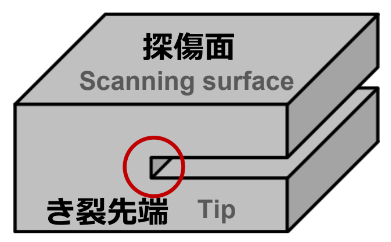
\includegraphics[width=100truemm,clip]{fig/実験I.png}
    \caption{Shape of the specimen in Experiment I.}
    \label{fig:実験I}
\end{figure}
\begin{figure}[htbp]
    \centering %中央揃え
    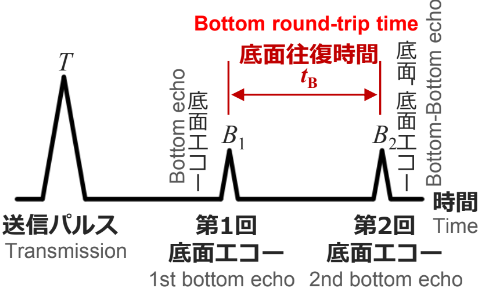
\includegraphics[width=100truemm,clip]{fig/試験体厚さ.png}
    \caption{Measurement of specimen thickness.}
    \label{fig:試験体厚さ}
\end{figure}
\begin{figure}[htbp]
    \centering %中央揃え
    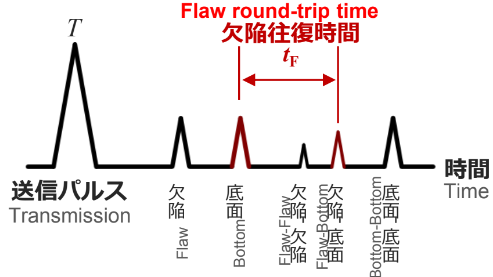
\includegraphics[width=100truemm,clip]{fig/欠陥深さ.png}
    \caption{Measurement of defect depth.}
    \label{fig:欠陥深さ}
\end{figure}
\begin{equation}
    \label{eq:試験片厚さ}
    z_B = \frac{1}{2}Ct_B
\end{equation}
\begin{equation}
    \label{eq:欠陥深さ}
    z_F = \frac{1}{2}Ct_F
\end{equation}

\subsection{実験II}
実験IIでは試験片Al1,Al2,ステンレスの3種類に対して測定を行った.実験手順を以下に示す.

\begin{enumerate}
    \item 実験Iと同様にしてそれぞれの試験片で,底面エコー高さ$B(V)$と底面往復時間を測定した.Al1を2回,Al2とステンレスを1回ずつ測定し,それぞれの平均を求めた.
    \item 底面往復時間$t_B$より試験片の厚さ$Z_B$を求めた.
    \item 求めた$z_B$より底面までの音波路程$n_B$を式(\ref{eq:音波路程})から計算した.ここで波長$\lambda$は$\lambda = C/f$である.
    \item 求めた$n_B$と図\ref{fig:AVG線図}から読み値$= 20log_{10} \frac{B}{B_0}$より,基準化したエコー高さ$B_0$を求めた.
    \item 次にAl1のき裂3点において,欠陥の位置$x, y$,欠陥エコー高さ$F$(V),欠陥往復時間$t_F$を測定した.3点目の欠陥のみ2回測定した.
    \item Al2及びステンレスは4つの欠陥においてAl1と同様に測定を行った.
    \item 測定結果から欠陥深さ$z_F$,欠陥エコー高さ$F$,欠陥音波路程$n_F$を計算した.さらに$F/B_0$を計算し,図\ref{fig:AVG線図}からGを過大評価により求め,式(\ref{eq:欠陥直径})より欠陥直径$d$を推定した.
\end{enumerate}
\begin{equation}
    \label{eq:音波路程}
    n_B = \frac{4z_B\lambda}{D^2}
\end{equation}
\begin{equation}
    \label{eq:欠陥直径}
    d = G \cdot D
\end{equation}

\subsection{実験III}
実験IIIでは,図\ref{fig:超音波映像装置}に示すような超音波映像装置による最先端の超音波技術により,ICカードの回路構造が表示される様子を観察した.

\begin{figure}[htbp]
    \centering %中央揃え
    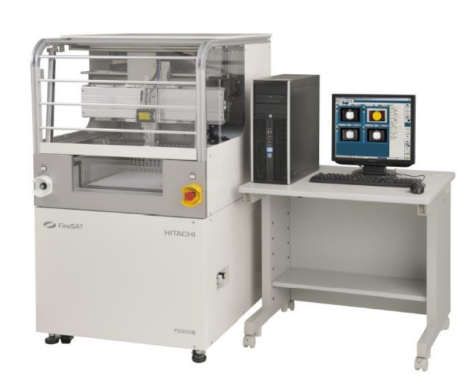
\includegraphics[width=100truemm,clip]{fig/超音波映像装置.png}
    \caption{Ultrasonic imaging device.}
    \label{fig:超音波映像装置}
\end{figure}